%&tex
\documentclass{article}

\usepackage[a4paper,margin=1in]{geometry}

\usepackage{graphicx}

\usepackage{amsmath}
\usepackage{cleveref}
\usepackage{subcaption}
\usepackage{bm}

\usepackage[backend=bibtex]{biblatex}
\addbibresource{supportingFiles/00_bibEntries/bibEntries.bib}

\title{Building Physics-Informed Neural Networks from scratch}
\author{Ramkumar}

\begin{document}

\maketitle

\tableofcontents

\begin{abstract}
	A physics-informed neural network (PINN in short) is an artificial neural
	network that learns the function from mathematical constraints that govern
	the underlying physics to be modelled. In this work, a PINN was built from
	scratch using Python programming language with fundamental libraries as
	numpy, pandas and matplotlib.  Aim of the present work is to get
	fundamental understanding on how a PINN works from the mathematical  and
	programming points of view.  Here, the classical fully connectected neural
	networks was constructed and tested by approximating a simple parabola plot
	data.  Further, the built network was developed to be physics-informed and
	validated by solving the ODE governing the exponential velocity decay of
	fluid due to viscosity. The understanding gained will be extended in
	further scientific computing using NNs.
\end{abstract}

\section{Introduction to neural networks}
\par{}
Machine learning is a branch of mathematics and computer science that develops
mathematical models that learn and mimic the human behavior. Deep learning
is a subset of machine learning that deals with artificial neural networks.\\
\par{}
A neuron is a mathematical function that takes in multiple weighted inputs
and returns a single output. It is similar to a biological neuron in terms
of connectivity and activation. Mathematically, it is represented as below.
\begin{align*}
	f_{neuron} = \sigma\left( \bm{w}^T.\bm{x} + b\right)
\end{align*}
\par{}
Here, \(\bm{x}\) is the input vector to the neuron and \(\bm{w}\) is its
corresponding weights vector. \(b\) is the bias of the neuron and \(\sigma\)
is the activation function.\\

\par{}
A Neural network is a set of inter-connected mathematically modelled neurons
that can work as a function approximator. It based on the
universal approximation theorm \cite{cybenko1989approximation} which states
as, any mathematically represented function \(f(x)\) can be approximated
by a neural network \(G(x)\) of sufficiently wide and deep to the tolerance \(\epsilon\).
Mathematically,
\begin{align*}
	| G(x) - f(x) | < \epsilon
\end{align*}

\par{}
Today, neural networks are of many types, but the fundamental ones are of three:
fully connected network, convolutional neural network, and reccurrent neural network,
with each serving a specific purpose. Fully connected network, also called as
dense network, is a set of layers of neurons in which each neuron on each layer
will be connected to all other neurons on nearby layers. They are good in
approximating the functions that invovle scalar IO variables. Convolutional
neural networks are best for the field data IOs, and the reccurrent type networks
are suitable for data that are of sequencial type. \\

\par{}
In the present work, the fully connected neural network is developed from
scratch and later it was turned into physics informed network. The mathematical
background, and the problems solved with the developed network were discussed
in the upcoming sections. \\


\section{Mathematical view on network training}
\par{}
Consider an example network shown in \cref{example_network}. Here, the input
data \(x\) is fed to a fully connected network that estimates the output
data \(\hat{y}\), which then compared with the expected output data \(y\) through
loss function.  \\

\begin{figure}
    \center
    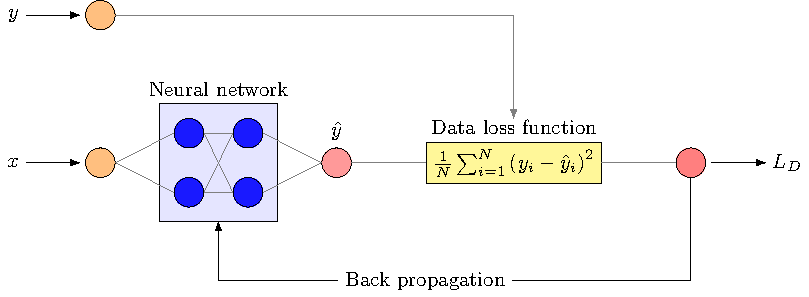
\includegraphics[scale=1]{supportingFiles/01_schematics/01_NN_example/NN_example.pdf}
    \caption{Example network}
    \label{example_network}
\end{figure}

\par{}
Weights and biases of the example network were then optimized with loss as
objective function, minimizing it to match the expected output values through
an algorithm called back propagation. The main reference for this back
propagation equations for a fully connected network is
\cite{backpropagation_reference}. \\

\par{}
Mathematically, a single layer \(l\) is represented as given below.
\begin{align*}
    \bm{x}^{[l]} = \sigma\left( \bm{z}^{[l]}\right)
\end{align*}

where,
\begin{align*}
    \bm{z}^{[l]} = \bm{W}^{[l]}\cdot\bm{x}^{[l-1]} + \bm{b}^{[l]}
\end{align*}

Here, \(\bm{W}^{[l]}\) is the weight matrix and \(\bm{b}^{[l]}\) is the bias
vector of layer \(l\).  \(\bm{x}^{[l-1]}\) is the activated output of the
previous layer \(l-1\), and \(\sigma\) is the activation function. Let, \(L\)
be the loss function evaluated at the end of last layer. Then, the gradient of
loss function with respect to the unactivated output of last layer\(z^{[l]}\)
is given as below.

\begin{align}
    \left.\frac{\partial L}{\partial \bm{z}^{[l-1]}} = \left[\bm{W}^{[l]} \right]^T \cdot \frac{\partial L}{\partial \bm{z}^{[l]}} * \frac{\partial \sigma}{\partial \bm{z}}\right\vert_{[l-1]} \label{error_eqn}
\end{align}

\Cref{error_eqn} is called as the error of a layer. The error is back
propagated from layer \(l\) to the previous layer \(l-1\) by the above
equation.  Here, \(*\) is the element-wise multiplication. To begin this back
propagation, we need the above error derivative \(\partial L/\partial z\) for
the last layer in the network. \\

\par{}
The computation of error for the last layer will involve the differentiation
of loss function \(L\) with respect to the estimated output \(\hat{y}\). Let
the last layer be described as given below.
\begin{align*}
    \bm{\hat{y}} = \sigma\left(\bm{z}\right)
\end{align*}

And, let the loss function be the classical mean squared error as given below.
\begin{align*}
    L = \frac{1}{N}\sum_{i=1}^{N} \left(\hat{y}_i - y_i\right)^2
\end{align*}

Then, the error for the last layer is calculated as shown below.
\begin{align*}
    \left.\frac{\partial L}{\partial \bm{z}}\right\vert_{[l]} = \frac{\partial L}{\partial \bm{\hat{y}}} \cdot \frac{\partial \bm{\hat{y}}}{\partial \bm{z}} = \frac{\partial L}{\partial \bm{\hat{y}}} \cdot \frac{\partial \sigma}{\partial \bm{z}} = \left(\frac{2}{N}\sum_{i=1}^{N}\left(\hat{y}_i - y_i\right)\right) \left.\frac{\partial \sigma}{\partial \bm{z}}\right\vert_{[l]}
\end{align*}

Hence, the above equation completes the error computation for all the layers, next
we have to compute the derivatives of loss with respect to weights and
biases of all the layers using these error vectors. The gradients of loss with
respect to weights and biases are computed using the error vector for each layer
as shown below.
\begin{align}
    \frac{\partial L}{\partial \bm{W}^{[l]}} &= \frac{\partial L}{\partial \bm{z}^{[l]}} \cdot \left[\bm{x}^{[l-1]}\right]^T \label{weight_eqn} \\
    \frac{\partial L}{\partial \bm{b}^{[l]}} &= \frac{\partial L}{\partial \bm{z}^{[l]}} \label{bias_eqn}
\end{align}

So, with the above gradient equations \cref{error_eqn,weight_eqn,bias_eqn}, the
weights and biases of all the layers can be computed and optimized with aim of
minimizing the loss function. An example problem with data-driven network is
given below that was solved with the neural network built using above
equations.


\section{Validating neural network code}
\par{}
A couple of datasets were chosen for validating the developed neural network
code. First is a simple parabola curve data that the network has to approximate
and the second one will be a normalized flight velocity profile data which
the network code has also to approximate. Each problem was explained in detail
as below. \\

\subsection{Parabola problem}
\par{}
The problem framed was to approximate the parabola curve defined with equation
\(y = x^2\) with \(x \in [0,0.5]\).\\

\par{}
A network with three layers and single neuron on each layer, i.e. two hidden
layers and one output layer, was built for this problem. The \(\tanh()\) is
used as the activation function for all the layers and \(mse\) is used as the
loss function for the network. The schematic of network for this problem is
given in \cref{parabola_network_schematic}.\\

\begin{figure}
   \center
    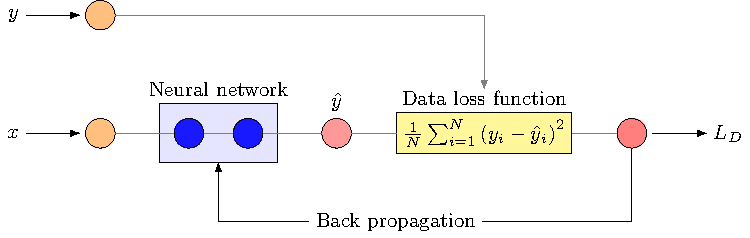
\includegraphics[scale=1]{supportingFiles/01_schematics/02_parabola_network/parabola_network.pdf}
    \caption{Neural network schematic for parabola problem}
    \label{parabola_network_schematic}
\end{figure}

\par{}
Training was performed on the generated data, and the resulting estimated
vs exact profiles were shown in \cref{parabola_result}. It can be seen that the
estimated result is accurate enough to approximate the \(y=x^2\) equation
within the range \(x,y \in [0,0.5]\). Accuracy analysis were not performed as the
motive is to check if the network code works. \\

\begin{figure}
   \center
    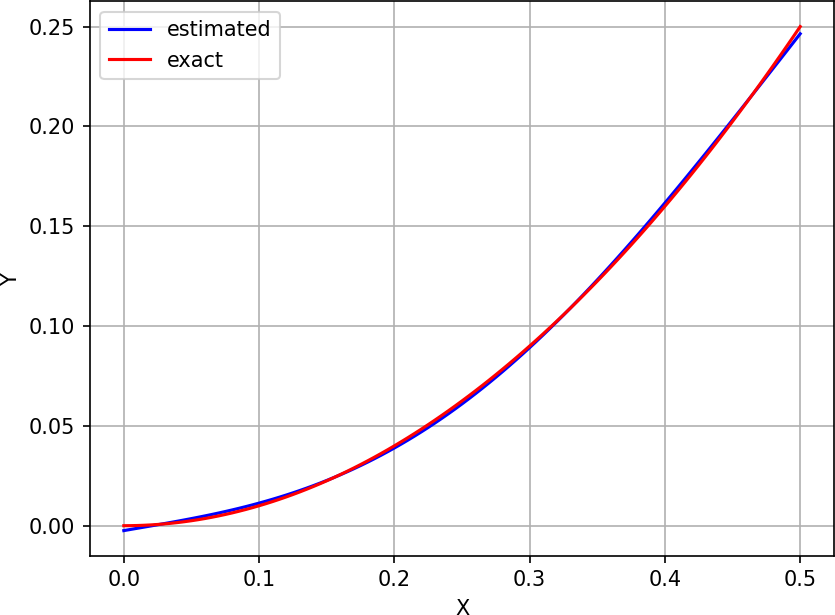
\includegraphics[scale=0.7]{supportingFiles/02_results/01_parabola_datadriven/estimation.png}
    \caption{Estimated vs exact parabola profile by the built neural network}
    \label{parabola_result}
\end{figure}


\subsection{Flight velocity profile}
\par{}
Second validation was performed using a flight velocity profile that was obtained
from the flight dynamics simulation done for an academics assignment work.
The profile was smooth and have both positive and negative curvatures, hence
chosen for the work. \\

\par{}
Schematic of the neural network built for this approximation was shown in
\cref{velocity_profile_network}. The network has 5 neurons with 3 hidden layers
and 1 neuron for the output. Same \(tanh()\) activation function was used
in all the layers. \\

\begin{figure}
   \center
    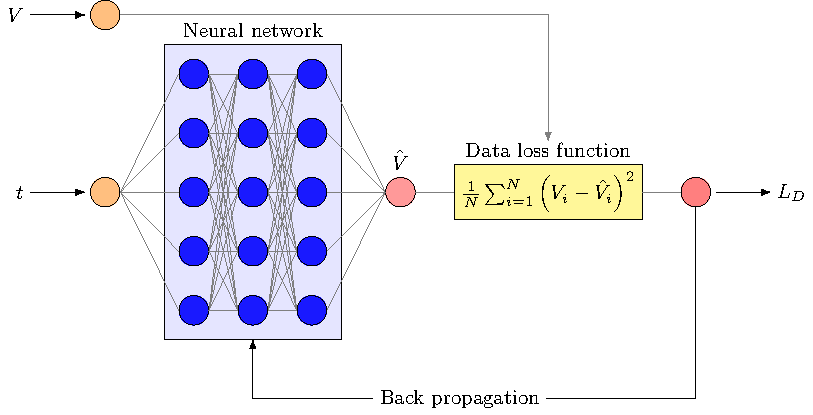
\includegraphics[scale=1]{supportingFiles/01_schematics/03_velocity_profile_network/velocity_profile.pdf}
    \caption{Neural network schematic of flight velocity profile problem}
    \label{velocity_profile_network}
\end{figure}

\par{}
The estimated vs exact flight velocity profiles were given in \cref{velocity_profile_output}.
It can be seen that the estimation matches pretty well with the exact velocity
profile, proving that the network code is correct. Thus, the next step of
enhancing the code to include physics information was performed. \\

\begin{figure}
   \center
    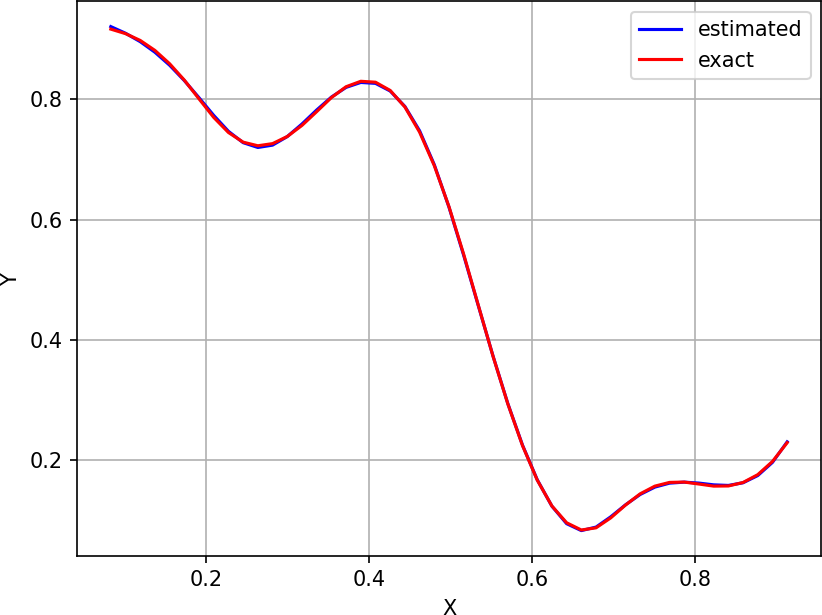
\includegraphics[scale=0.7]{supportingFiles/02_results/02_velocity_profile_dataDriven/estimation.png}
    \caption{Estimated vs exact flight velocity profiles, here X is \(t\) and Y is \(V\)}
    \label{velocity_profile_output}
\end{figure}



\section{Enhancing network with physics information}
\par{}
The already developed neural network code was validated against two dataset,
and now the code has to be enhanced to include physics information in the form
of mathematical constraints.\\

\par{}
For each problem to be solved with this network code, the code has to be
modified to include the mathematical constraints in the last layer or so. The
mathematical constraints can be of two types, either algebraic or differential
equations. Algebraic equations involving output and input variables can be
directly coded, but, coding the differential equations will require the
derivatives to be computed using automatic differentiation in the network which
was accomplished as explained below.\\

\subsection{Computing derivatives output w.r.t input}
\par{}
The differential equations (ODEs and PDEs) will involve the
derivatives of dependent variables w.r.t. independent variables. In the
network terms, the dependent variables are the output variables and the
independent ones are the input variables. Thus, as similar to the loss derivative
equations, an equation for computing derivative of a layer output w.r.t. its
input was derived. \\

\par{}
Keeping backpropagation equations as base idea, the matrix equation for
\(\partial \sigma/\partial x\) of a layer was propertly derived and is given
below as.

\begin{align}
    \left[\frac{\partial \sigma}{\partial \bm{x}}\right] = \left[\bm{W}\right]^T \cdot diag\left(\frac{\partial \sigma}{\partial \bm{z}}\right) \label{differential_matrix_eqn}
\end{align}

\par{}
Here, \(\partial \sigma/\partial x\) is a vector of the layer and
\(diag\left(\partial \sigma/\partial x\right)\) is a diagonal matrix with those
vector elements on the diagonal.\(\left[\frac{\partial \sigma}{\partial
\bm{x}}\right] \) is a mtrix of same size as of \(\left[\bm{W}\right]^T\). \\

\par{}
It has to be noted that the \cref{differential_matrix_eqn} gives derivative
of output with respect to input of a single layer only. The chain rule in
differential calculus has to be used to get the derivative of overall output
of the network to its actual input.\\

\subsection{Validating the gradient equation}
\par{}
The matrix equation \cref{differential_matrix_eqn} was validated for it working
by testing it on the network that was trained based on pure data. A network
was built and trained using a synthetic data of fluid velocity decay at a point
in flow due to fluid viscosity. The synthetic data was generated using below equation
with \(k = 5.0\) and \(V_0 = 1\).

\begin{align*}
    V(t) = V_0 e^{-k t}
\end{align*}

And its corresponding ODE for derivative computation is given below.

\begin{align*}
    \frac{d V}{d t} = -k V
\end{align*}

\par{}
The network was trained for \(X = t = [0,0.5]\) and its corresponding velocity
values. The estimated vs exact velocity decay profile is given in
\cref{validation_decay_profile}.  And then, the trained layer weights were used
to compute the derivative \(d V/d t\) which were compared to the exact values
and given in \cref{validation_derivative_profile}.  It can be seen that the
derivative profiles match quite well except at the beginning which is due to
limitation in approximating the velocity profile, and that was later rectified
in validating the PINN network. Thus, the derivative computation is validated,
and next step will be to validate the self built physics-informed neural
network.

\begin{figure}
    \begin{subfigure}{0.5\linewidth}
       \center
        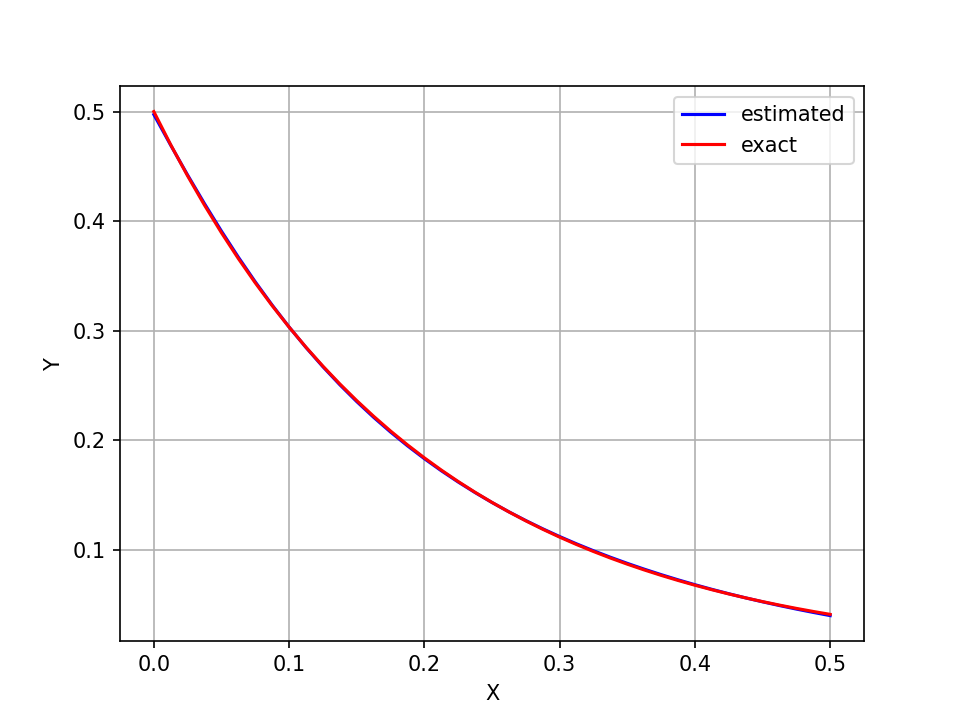
\includegraphics[scale=0.5]{supportingFiles/02_results/03_derivative_validation/estimation.png}
        \caption{Velocity profile estimated vs expected}
        \label{validation_decay_profile}
    \end{subfigure}
    \hfill
    \begin{subfigure}{0.5\linewidth}
       \center
        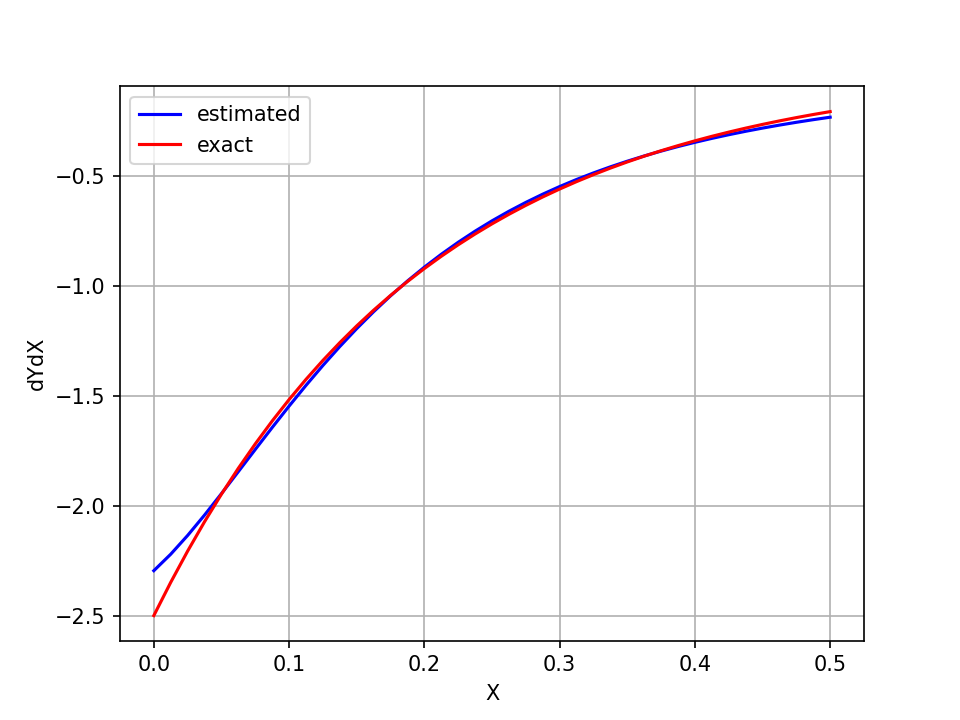
\includegraphics[scale=0.5]{supportingFiles/02_results/03_derivative_validation/derivative.png}
        \caption{\(dV/dt\) profile estimated vs expected}
        \label{validation_derivative_profile}
    \end{subfigure}
    \hfill
    \caption{Validation graphs for derivative computation}
\end{figure}



\section{Validating Physics-Informed Neural Network (PINN) code}
\par{}
Validating the enhanced PINN code was done with two chosen problems. First one
is to approximate the same parabola profile but with equation \(y=x^2\) instead
of y-data, and the second one is to model the fluid velocity decay profile due
to fluid viscosity, which involves differential equation. \\

\subsection{Parabola profile with equation}
\par{}
The problem is similar to the one used for validating the neural network code
earlier, except the fact that, the y-data is made unavailable and the
governing equation \(y=x^2\) is given instead. The residual of the equation
will be given to the loss function which has to be minimized for training the
model. The network architecture is given in \cref{parabola_PINN_network}.
And the estimated vs expected results graph is given in \cref{parabola_PINN_result}.\\

\begin{figure}
   \center
    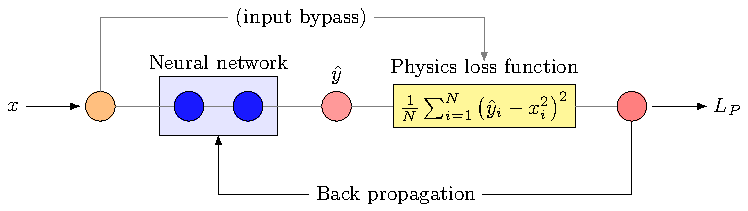
\includegraphics[scale=1]{supportingFiles/01_schematics/04_parabola_PINN_network/parabola_PINN.pdf}
    \caption{PINN network schematic for parabola problem}
    \label{parabola_PINN_network}
\end{figure}

\begin{figure}
   \center
    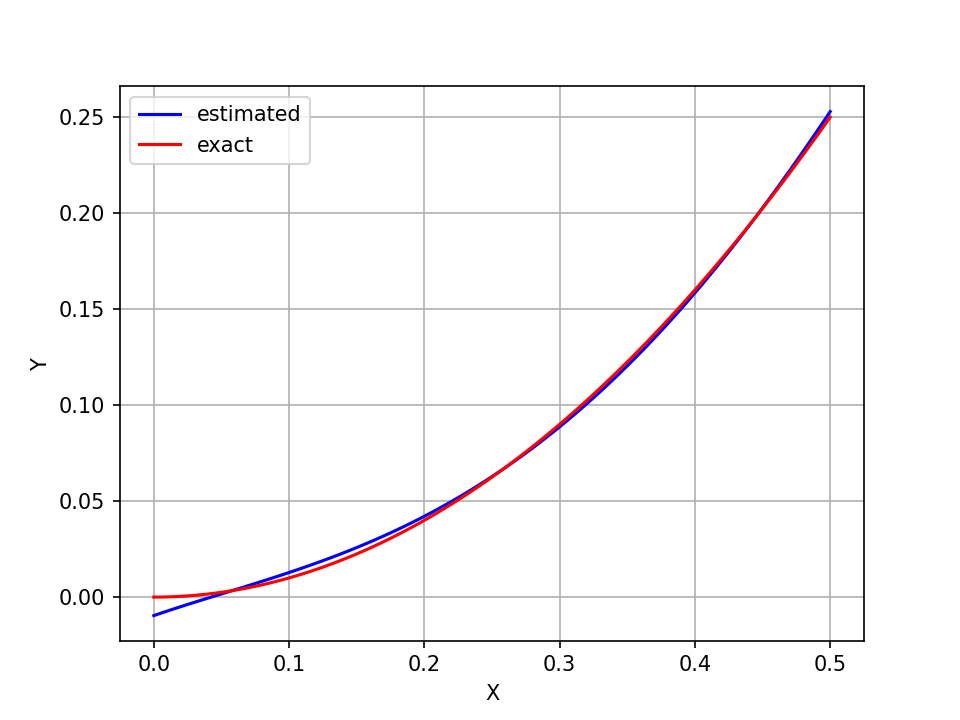
\includegraphics[scale=0.7]{supportingFiles/02_results/04_parabola_PINN/estimation.png}
    \caption{Parabola estimated vs exact result using PINN}
    \label{parabola_PINN_result}
\end{figure}

\subsection{Exponential velocity decay due to fluid viscosity}
\par{}
Given a point in a free fluid flow, the velocity of fluid particles will decay
at the point due to the resistance termed as fluid viscosity. This decay
will be in exponential form and is governed by \cref{velocity_decay_equation},
which was already discussed partially in the derivative validation section.

\begin{align}
    \frac{d V}{d t} = -k V \label{velocity_decay_equation}
\end{align}

Here, \(k\) is a constant denoting fluid viscosity.
The equation is of autonomous form and has analytical solution given as below.

\begin{align*}
    V = V_0 e^{-k t}
\end{align*}

\(V_0\) is the initial velocity of the fluid flow. Schematic of the PINN used
for the problem is given in \cref{velocity_decay_PINN_schematic}. Here, the
network has two hidden layers with 3 and 2 neurons respectively, and an
output layer with 1 neuron. \(tanh()\) activation function was used in all
the layers.\\

\begin{figure}
   \center
    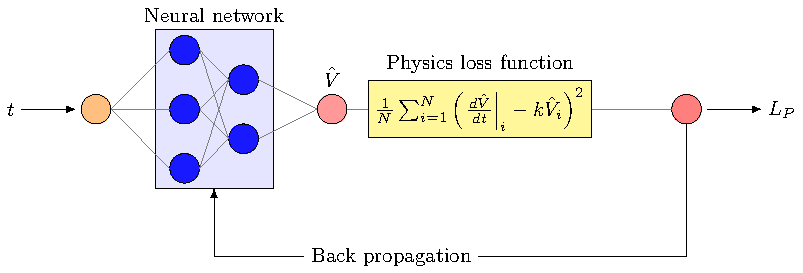
\includegraphics[scale=1]{supportingFiles/01_schematics/05_velocity_PINN_network/velocity_PINN.pdf}
    \caption{Velocity decay problem PINN schematic}
    \label{velocity_decay_PINN_schematic}
\end{figure}

\par{}
The loss function of this network is made in two parts, the first part will enforce
the initial condition of velocity and will be made active only at the starting
of time data, it is given as below.
\begin{align}
    L_{IC} = \left.\left(\hat{V}_i - V_i\right)^2\right|_{t=0, i=0} \label{IC_eqn}
\end{align}

The second part will contain the governing equation constraint and that will be
executed for all timesteps. The equation is as given below.

\begin{align}
    L_{ODE} = \frac{1}{N}\sum_{i=0}^{N}\left(\left.\frac{d\hat{V}}{dt}\right\vert_i - k\hat{V}_i\right)^2 \label{ODE_eqn}
\end{align}

So, the total loss function for the network will be sum of \cref{IC_eqn,ODE_eqn},
as given below.
\begin{align}
    L = L_{IC}+L_{ODE} =  \left.\left(\hat{V}_i - V_i\right)^2\right|_{t=0, i=0}+\frac{1}{N}\sum_{i=0}^{N}\left(\left.\frac{d\hat{V}}{dt}\right\vert_i - k\hat{V}_i\right)^2 \label{velocity_decay_LF}
\end{align}

Actually, to increase the weightage of initial condition as it is active only
in a part of the back propagation, a factor of 10 was multiplied to its compontent
and the final loss equation is given as below.
\begin{align}
    L = L_{IC} \times 10+L_{ODE} \label{velocity_decay_PINN_LF}
\end{align}

\par{}
The model was trained successfully, and the estimated results of velocity
profile and the derivative computation were given in
\cref{velocity_decay_PINN_results}.  It was found that the derivative estimated
was accurate than the one shown for the validation. This is because the network
that learns a function through physics constraints learn better than the
network that maps the same function through data. \\

\begin{figure}
    \begin{subfigure}{0.5\linewidth}
       \center
        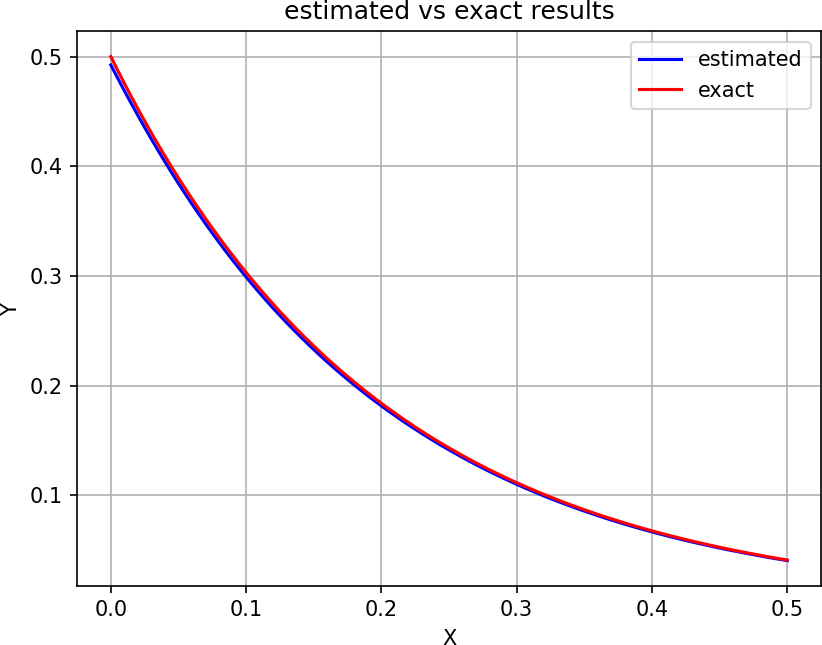
\includegraphics[scale=0.5]{supportingFiles/02_results/05_velocity_decay/estimated_output.png}
        \caption{Estimated vs expected velocity decay profile, (here X = t, Y = V)}
        \label{}
    \end{subfigure}
    \hfill
    \begin{subfigure}{0.5\linewidth}
       \center
        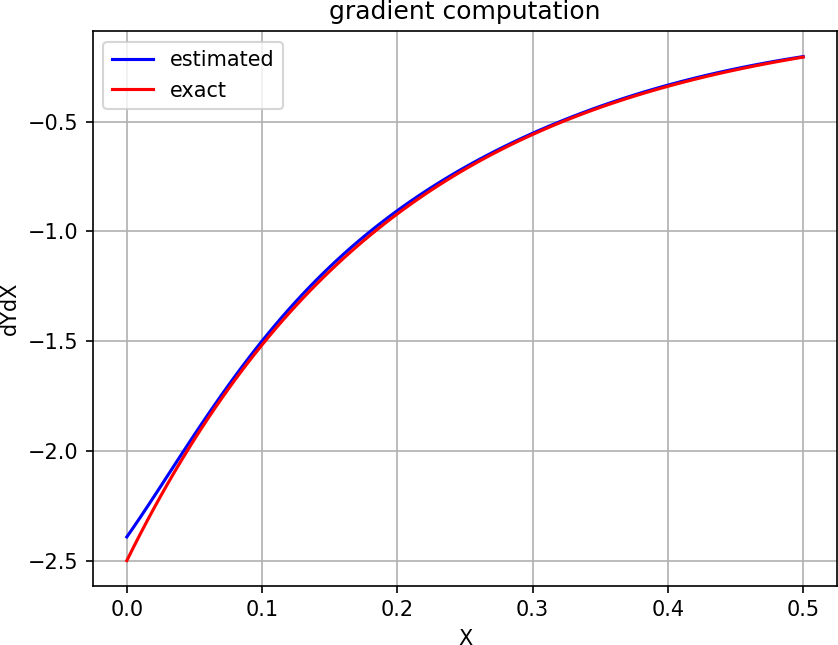
\includegraphics[scale=0.5]{supportingFiles/02_results/05_velocity_decay/gradient_computation.png}
        \caption{Estimated vs expected gradient profile, (here X = t, Y = V)}
        \label{}
    \end{subfigure}
    \caption{Exponential velocity decay due to fluid viscosity problem solution using PINNs}
    \label{velocity_decay_PINN_results}
\end{figure}

\par{}
The error percentage graph for the estimated vs expected velocity profiles
was given in \cref{velocity_PINN_EP_graph}. The error percentage were in the
order of 1-2\%, hence this validates the PINN code developed.

\begin{figure}
   \center
    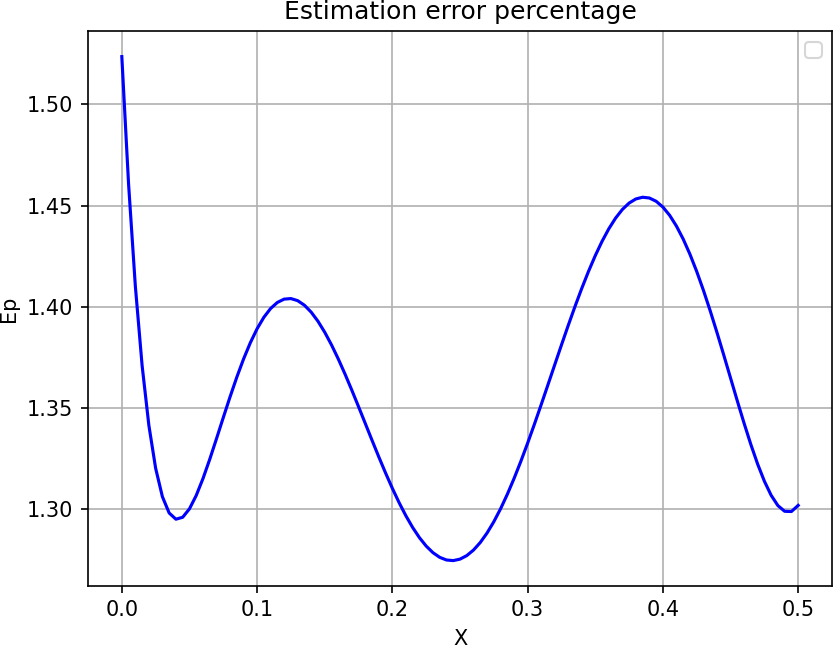
\includegraphics[scale=0.7]{supportingFiles/02_results/05_velocity_decay/error_percentage.png}
    \caption{Error percentage of estimated vs expected velocity profiles}
    \label{velocity_PINN_EP_graph}
\end{figure}


\section{Python code structure}
\par{}
In each of the source code that was provided with this documentation,
there will be 3 python scripts, each handling specific part of the program.
They are as listed below.
\begin{itemize}
    \item script\_main.py
    \item inputData.py
    \item customLayers.py
\end{itemize}

\par{}
The \textit{script\_main.py} is the main script that constructs the network and
has snippets related to physics information. \textit{inputData.py} script
contains the snippets that determine the input parameters, such as number of
layers and neurons on them, whether to save/load weights and learning rate
adaptation code. Finally, \textit{customLayers.py} contains the class
definition of a neural network layer that has everything related to layers such
as activation function, its derivative and forward evaluation. Activation function
is hard coded for now, and later may be made generalizable. \\

\par{}
The code was made as generalizable in terms of having number of neurons/layers
for now, and the code is for fully connected dense network. Later, the future
work may include custom codes for other network types when the need arises. \\


\section{Conclusion and future works}
\par{}
I conclude the present work by stating that a high level of understanding and
knowledge gained in the perspective of mathematics and programming of neural
networks, that opened gateways for other methods of using neural networks,
such as optimizing input values itself based on loss to find optimal
values etc... The present work is limited to the generalization code of
fully connected dense network. And, this code may be extended for other
scientific computation uses such as Neural ODEs.


\printbibliography

\end{document}

